\documentclass{beamer}
\usepackage{epstopdf}
\usepackage{adjustbox}
\usepackage{tikz}
\usetikzlibrary{
	positioning				% Allows 5px above/below of x style positioning
	, arrows				% Allows <-, ->, <-> style arrows.
	, fit					% Allows fitting lines to shapes
	, decorations.pathreplacing	% Allows decoration that affect line paths.
	, backgrounds
	, shapes
	, shapes.multipart
	, calc
	, chains
}
\usepackage{todonotes}

\mode<presentation> {
	\usetheme{Malmoe}
	\usecolortheme{whale}
	\setbeamertemplate{footline}[page number]
	\setbeamertemplate{navigation symbols}{}
}

%----------------------------------------------------------------------------------------
%	TITLE PAGE
%----------------------------------------------------------------------------------------

\title[Short title]{Project NUClear}

\author{
	Trent Houliston \and Jake Woods \and Joshua Kearns \and Michael Burton
}

\institute[UoN]
{
	University of Newcastle \\ % Your institution for the title page
	\medskip
	\textit{Trent.Houliston@uon.edu.au, Jake.f.woods@gmail.com} % Email address
}

\date{\today}

% Start of document
\begin{document}

%----------------------------------------------------------------------------------------
% Title Slide 
%----------------------------------------------------------------------------------------
\begin{frame}
	\titlepage % Print the title page as the first slide
\end{frame}

%----------------------------------------------------------------------------------------
% Overview (Table of Contents)
%----------------------------------------------------------------------------------------
\begin{frame}
	\tableofcontents
\end{frame}

%----------------------------------------------------------------------------------------
\section{Introduction}
%----------------------------------------------------------------------------------------
\begin{frame}
\end{frame}

\begin{frame}
	\frametitle{Problem Description}
		Improve the software architecture of the NUbots robocup system to:
		\begin{itemize}
			\item Facilitate the use of robots for research, marketing, other non-soccer based behaviours.
			\item Improve the time it takes to become effective with the NUbots code.
			\item Make it easier to take full advantage of the robots hardware.
		\end{itemize}
\end{frame}

\begin{frame}
	\frametitle{Estimated Effort}
		Time \& Money
		\begin{itemize}
			\item 48 person-months of effort.
			\item Estimated cost of \$200,000 (using COCOMO)
		\end{itemize}
		
		Additional Factors
		\begin{itemize}
			\item Loss of team members
			\item Required a large set of companion documentation
		\end{itemize}
\end{frame}

%----------------------------------------------------------------------------------------
\section{Existing System}
%----------------------------------------------------------------------------------------
\begin{frame}
	\sectionpage
\end{frame}

\begin{frame}
	\frametitle{Existing System}
	\begin{itemize}
		\item The NUbots system has an existing system
	\end{itemize}
\end{frame}

\begin{frame}
	\frametitle{Existing Architecture}
	\begin{itemize}
		\item The system runs in a synchronised dual pipeline architecture
			\begin{itemize}
				\item The See Think loop holds most of the logic and decision making code
				\item The Sense Move loop is a much smaller loop that simply reads from the sensor and camera, and writes motor actions to the motors
			\end{itemize}
		\item The threads are synchronised to run at regular intervals
		\item Most of these systems read in from the Blackboard and write back to it
		\item Some of them will communicate using a message system called Jobs
		\item The remainder of the communication is done using direct function calls on singletons
	\end{itemize}
\end{frame}

\begin{frame}
	\frametitle{Existing Architecture - Data Flow Diagram}
	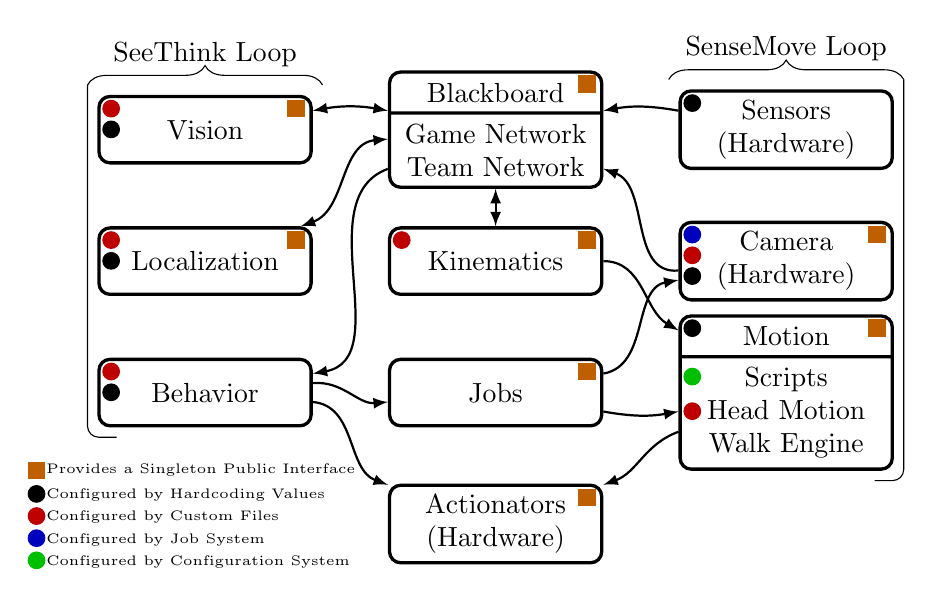
\begin{tikzpicture}[
			x=10.5em,y=4.75em,
			component/.style={
				rectangle
				, rounded corners
				, draw=black, very thick
				, text width=7em
				, minimum height=2.4em
				, text centered
			}
			, splitcomponent/.style={
				component
				, rectangle split
				, rectangle split parts=2
			}
			, configsystemconfig/.style={ color=green!75!black }
			, fileconfig/.style={ color=red!75!black }
			, jobconfig/.style={ color=blue!75!black }
			, hardcodedconfig/.style={ color=black }
			, publicinterface/.style={ color=orange!75!black}
			, write/.style={ ->, thick}
			, read/.style={<-, thick}
			, readwrite/.style={<->, thick}
			, >=latex
		]

		%\node at (0.5,2.5) {$P_{1}$};

		%%% Nodes
		%% Left hand Side
		\node at (0,3) [component] (vision) {Vision};
		\node at (0,2) [component] (localization) {Localization};
		\node at (0,1) [component] (behavior) {Behavior};

		%% Center
		\node at (1, 3) [splitcomponent] (blackboard) {Blackboard \nodepart{two} Game Network\\Team Network};
		\node at (1, 2) [component] (kinematics) {Kinematics};
		\node at (1, 1) [component] (jobs) {Jobs};
		\node at (1, 0) [component] (actionators) {Actionators (Hardware)};

		%% Right hand side
		\node at(2,3) [component] (sensors) {Sensors (Hardware)};
		\node at(2,2) [component] (camera) {Camera (Hardware)};
		\node at(2,1) [splitcomponent] (motion) {Motion \nodepart{two} Scripts\\Head Motion\\Walk Engine};

		%%% Connections
		%% Left side connections
		\path [readwrite, out=10, in=170] (vision) edge (blackboard);
		\path [readwrite, out=20, in=185] (localization) edge (blackboard);
		\path [read, out=10, in=200] (behavior) edge (blackboard);
		\path [write, out=5, in=185] (behavior) edge (jobs);
		\path [write, out=-5, in=160] (behavior) edge (actionators);
		
		%% Center connections
		\path [readwrite] (kinematics) edge (blackboard);

		%% Right side connections
		\path [write, out=170, in=10] (sensors) edge (blackboard);
		\path [write, out=185, in=-20] (camera) edge (blackboard);
		\path [write, out=-10, in=190] (jobs) edge (motion);
		\path [write, out=10, in=190] (jobs) edge (camera);
		\path [write, out=200, in=20] (motion) edge (actionators);
		\path [read, out=150, in=0] (motion) edge (kinematics);
		
		%%% Configuration Colours
		%% Vision
		\filldraw[fileconfig] ([yshift=-.5em,xshift=.5em]vision.north west) circle (3pt);
		\filldraw[hardcodedconfig] ([yshift=-1.25em,xshift=.5em]vision.north west) circle(3pt);
		\filldraw[publicinterface] ([yshift=-.8em,xshift=-0.9em]vision.north east) rectangle ++(6pt, 6pt);	
		
		%% Localization
		\filldraw[fileconfig] ([yshift=-.5em,xshift=.5em]localization.north west) circle(3pt);
		\filldraw[hardcodedconfig] ([yshift=-1.25em,xshift=.5em]localization.north west) circle (3pt);
		\filldraw[publicinterface] ([yshift=-.8em,xshift=-0.9em]localization.north east) rectangle ++(6pt, 6pt);
		
		%% Behavior
		\filldraw[fileconfig] ([yshift=-.5em,xshift=.5em]behavior.north west) circle(3pt);
		\filldraw[hardcodedconfig] ([yshift=-1.25em,xshift=.5em]behavior.north west) circle(3pt);
		
		%% Blackboard
		\filldraw[publicinterface] ([yshift=-.8em,xshift=-0.9em]blackboard.north east) rectangle ++(6pt, 6pt);
		
		%% Kinematics
		\filldraw[fileconfig] ([yshift=-.5em,xshift=.5em]kinematics.north west) circle(3pt);
		\filldraw[publicinterface] ([yshift=-.8em,xshift=-0.9em]kinematics.north east) rectangle ++(6pt, 6pt);
		
		%% Jobs
		\filldraw[publicinterface] ([yshift=-.8em,xshift=-0.9em]jobs.north east) rectangle ++(6pt, 6pt);
		
		%% Actionators
		\filldraw[publicinterface] ([yshift=-.8em,xshift=-0.9em]actionators.north east) rectangle ++(6pt, 6pt);
		
		%% Sensors
		\filldraw[hardcodedconfig] ([yshift=-.5em,xshift=.5em]sensors.north west) circle(3pt);
		
		%% Camera
		\filldraw[jobconfig] ([yshift=-.5em,xshift=.5em]camera.north west) circle(3pt);
		\filldraw[fileconfig] ([yshift=-1.25em,xshift=.5em]camera.north west) circle(3pt);
		\filldraw[hardcodedconfig] ([yshift=-2em,xshift=.5em]camera.north west) circle (3pt);
		\filldraw[publicinterface] ([yshift=-.8em,xshift=-0.9em]camera.north east) rectangle ++(6pt, 6pt);
		
		%% Motion
		\filldraw[hardcodedconfig] ([yshift=-.5em,xshift=.5em]motion.north west) circle (3pt);
		\filldraw[configsystemconfig] ([yshift=-2.25em,xshift=.5em]motion.north west) circle (3pt);
		\filldraw[fileconfig] ([yshift=-3.5em,xshift=.5em]motion.north west) circle(3pt);
		\filldraw[publicinterface] ([yshift=-.8em,xshift=-0.9em]motion.north east) rectangle ++(6pt, 6pt);
		
		%%% Legend
		\coordinate (legendpoint) at (.55, .35);
		
		%% Public Interface
		\node [below=3pt of legendpoint,anchor=south east] (publicinterfacelabel) {\tiny Provides a Singleton Public Interface};
		\filldraw[publicinterface] ([yshift=-3pt,xshift=-3pt]publicinterfacelabel.west) rectangle ++(6pt, 6pt);

		%% Hard Coded Config
		\node [below=0.9em of publicinterfacelabel.south west,anchor=south west] (hardcodedconfiglabel) {\tiny Configured by Hardcoding Values};
		\filldraw[hardcodedconfig] ([yshift=.5pt]hardcodedconfiglabel.west) circle (3pt);
		
		%% File Config
		\node [below=0.8em of hardcodedconfiglabel.south west,anchor=south west] (fileconfiglabel) {\tiny Configured by Custom Files};
		\filldraw[fileconfig] ([yshift=.5pt]fileconfiglabel.west) circle (3pt);

		%% Job Config
		\node [below=0.8em of fileconfiglabel.south west,anchor=south west] (jobconfiglabel) {\tiny Configured by Job System};
		\filldraw[jobconfig] ([yshift=.5pt]jobconfiglabel.west) circle (3pt);

		%% Config System Config
		\node [below=0.8em of jobconfiglabel.south west,anchor=south west] (configsystemconfiglabel) {\tiny Configured by Configuration System};
		\filldraw[configsystemconfig] ([yshift=.5pt]configsystemconfiglabel.west) circle (3pt);
		
		%%% Decorations
		%% SeeThink header
		\node[fit=(vision)(localization)(behavior)](leftgroup){};
		\draw[rounded corners] 
		(leftgroup.north west)--(leftgroup.south west) -- ++(0.10,0);			
		\draw[decorate,decoration={amplitude=7pt,brace}] % Header line
		(leftgroup.north west) -- (leftgroup.north east);

		\node[above=1.1em of leftgroup,anchor=center]{SeeThink Loop};

		%% SenseMove header
		\node[fit=(sensors)(camera)(motion)](rightgroup){};
		\draw[rounded corners] 
		(rightgroup.north east) -- (rightgroup.south east) -- ++(-0.10,0);
		\draw[decorate,decoration={amplitude=7pt,brace}]
		(rightgroup.north west) -- (rightgroup.north east);
		\node[above=1.1em of rightgroup,anchor=center]{SenseMove Loop};
	\end{tikzpicture}

\end{frame}

\begin{frame}
	\frametitle{Existing Architecture - Dependency Graph}
	\begin{adjustbox}{max totalsize={\textwidth}{.9\textheight},center}
	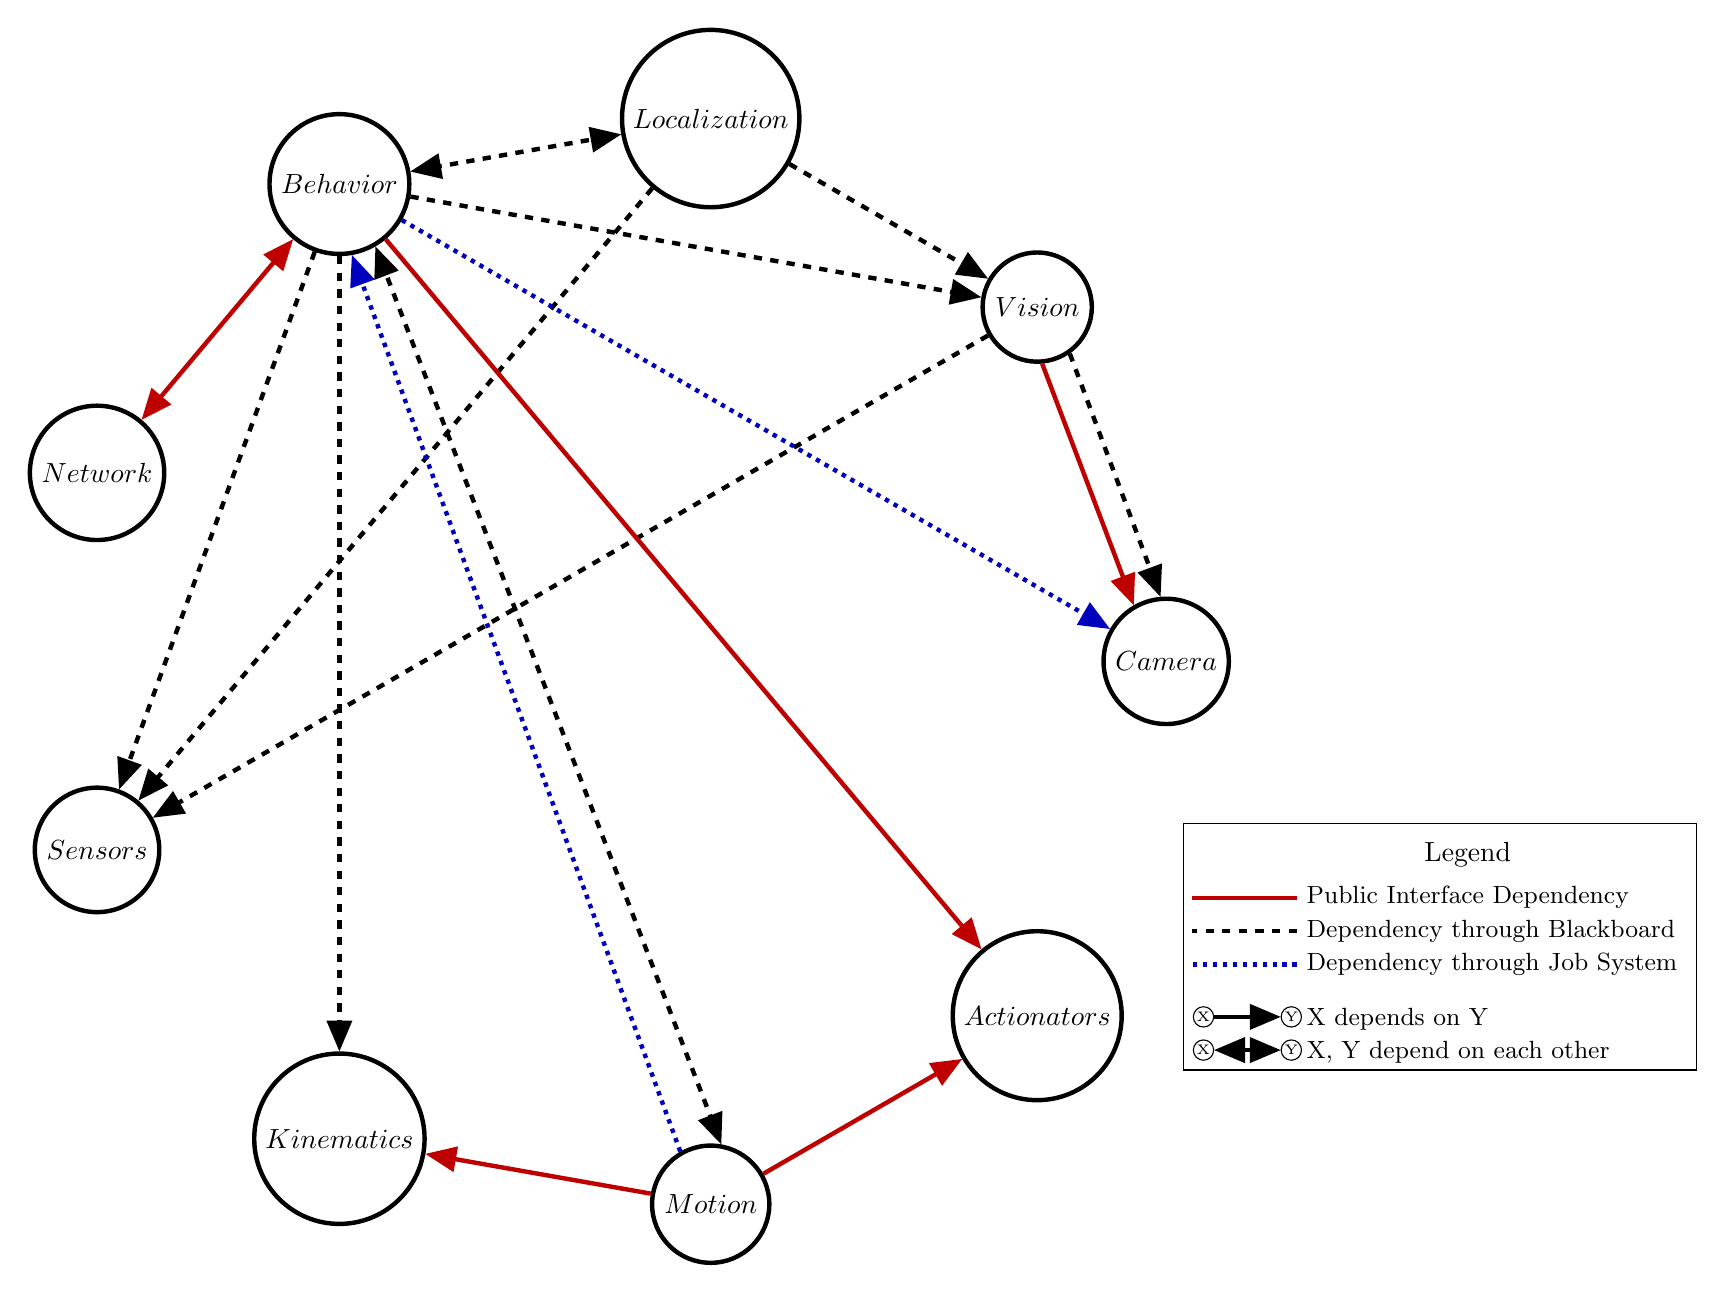
\begin{tikzpicture}[
		reactor/.style={draw, circle, ultra thick}
		, basearrow/.style={>=triangle 45, ultra thick}
		, blackboard/.style={basearrow, dashed}
		, publicinterface/.style={basearrow, color=red!75!black}
		, jobs/.style={basearrow, dotted, color=blue!75!black}
		, dependent/.style={->}
		, codependent/.style={<->}]

		%%% Legend
		\coordinate (legendpoint) at (13, -2);

		%% Public Interface Dependency
		\node [below=of legendpoint,anchor=east] (publicinterfacelabel) {\small Public Interface Dependency};
		\draw [publicinterface] (publicinterfacelabel.mid west) -- ++(-38pt, 0pt);

		%% Blackboard Dependency
		\node [below=12pt of publicinterfacelabel.south west,anchor=south west] (blackboardlabel) {\small Dependency through Blackboard};
		\draw[blackboard] (blackboardlabel.mid west) -- ++(-38pt, 0pt);

		%% Jobs Dependency
		\node [below=12pt of blackboardlabel.south west,anchor=south west] (joblabel) {\small Dependency through Job System};
		\draw[jobs] (joblabel.mid west) -- ++(-38pt, 0pt);

		%% Dependancy Type: Depends on
		\node[below=20pt of joblabel.south west,anchor=south west] (dependencylabel) {\small X depends on Y};
		\node[circle, draw, inner sep=0.5pt] (dependencynodeY) at ([yshift=1pt,xshift=-2pt]dependencylabel.mid west) {\tiny Y};
		\node[circle, draw, inner sep=0.5pt, left=24pt of dependencynodeY] (dependencynodeX) {\tiny X};
		\draw[basearrow, dependent] (dependencynodeX) edge (dependencynodeY);

		%% Dependancy Type: Codependent
		\node[below=12pt of dependencylabel.south west,anchor=south west] (codependencylabel) {\small X, Y depend on each other};
		\node[circle, draw, inner sep=0.5pt] (codependencynodeY) at ([yshift=1pt,xshift=-2pt]codependencylabel.mid west) {\tiny Y};
		\node[circle, draw, inner sep=0.5pt, left=24pt of codependencynodeY] (codependencynodeX) {\tiny X};
		\draw[basearrow, codependent] (codependencynodeX) edge (codependencynodeY);

		%% Legend Header
		\node[above=0pt of publicinterfacelabel] (legendheader) {Legend};

		%%% Draw all of our components in a circle
		\foreach [count=\i] \reactor in {Camera, Vision, Localization, Behavior, Network, Sensors, Kinematics, Motion, Actionators} {
		
			% Draw the reactors around the central star
			\node[reactor] (\reactor) at ({360/9 * (\i - 1)}:7cm) {$\reactor$};
		};

		%% Legend Border
		\node[fit=(legendheader)(publicinterfacelabel)(blackboardlabel)
				(joblabel)(dependencylabel)(codependencynodeX)(codependencynodeY),rectangle,draw](legendgroup){};

		%%% Dependencies
		%% Vision
		\path[blackboard, dependent] (Vision.305) edge (Camera.95);
		\path[publicinterface, dependent] (Vision.275) edge (Camera.120);
		\path[blackboard, dependent] (Vision) edge (Sensors);

		%% Localization
		\path[blackboard, dependent] (Localization) edge (Sensors);
		\path[blackboard, dependent] (Localization) edge (Vision);

		%% Behavior
		\path[blackboard, codependent] (Behavior) edge (Localization);
		\path[blackboard, dependent] (Behavior) edge (Kinematics);
		\path[blackboard, dependent] (Behavior) edge (Vision);
		\path[blackboard, dependent] (Behavior) edge (Sensors);
		\path[publicinterface, dependent] (Behavior) edge (Actionators);
		\path[publicinterface, codependent] (Behavior) edge (Network);
		\path[jobs, dependent] (Behavior) edge (Camera);

		%% Motion
		\path[blackboard, codependent] (Motion.80) edge (Behavior.300);
		\path[jobs, dependent] (Motion.120) edge (Behavior.280);
		\path[publicinterface, dependent] (Motion) edge  (Actionators);
		\path[publicinterface, dependent] (Motion) edge (Kinematics);
	\end{tikzpicture}
	\end{adjustbox}
\end{frame}

\begin{frame}
	\frametitle{Problems in Existing System}
	\begin{itemize}
		\item Hidden Dependencies
			\begin{itemize}
				\item The existing systems dependencies are very poorly defined
				\item For example, localizations dependency on the Stationary/Mobile object system.
				\item These hidden dependencies make it difficult to work on a system without understanding the whole system
			\end{itemize}
	
		\item Threading Issues
			\begin{itemize}
				\item Current system does not handle synchronisation between the two threads well
				\item e.g. The kick system can be prompted mid way by the walk engine, the two can even run together resulting in the robot standing still for prolonged periods.
				\item Happens because the interactions between the two threads is undefined in most cases
			\end{itemize}
	\end{itemize}
\end{frame}

\begin{frame}
	\frametitle{Problems in Existing System}
	\begin{itemize}			
		\item Network Communication
			\begin{itemize}
				\item Network communication is currently entirely through Localisation and Behaviour
				\item Adding new network communication requires modifying these two systems
				\item Because of the difficulty of adding new networking, no new networking will be added
			\end{itemize}
			
		\item Build System
			\begin{itemize}
				\item The current build system uses a make file that calls cmake that builds a make file that is called by the original make file
				\item This makes adding and removing components to the system in a meaningful way difficult
			\end{itemize}
	\end{itemize}
\end{frame}

\begin{frame}
	\frametitle{Wishlist}
	\begin{itemize}
		\item Modular Design
			\begin{itemize}
				\item Many modules that are made for robotics (walk engine, script engine) are useful for more then just soccer.
				\item Being able to use Mock inputs allows the system to be tested without access to a robot
				\item Being able to compose various modules into a binary would allow the robot to do more
				\item Enabling the sharing of these modules between researchers would result in better development (more people using the same code)
			\end{itemize}
			
		\item Transparent Multithreading
			\begin{itemize}
				\item Modern CPUs are getting more cores, rather then becoming faster
				\item Threading is difficult and can almost never be sensibly done at the module level
				\item Threading should be handled by the architecture in a way that can scale up to many cores
			\end{itemize}
	\end{itemize}
\end{frame}
			
\begin{frame}
	\frametitle{Wishlist}
	\begin{itemize}
		\item Runtime Statistics
			\begin{itemize}
				\item When optimising programs for speed it is useful to see how long each section of the code took
				\item Breaking up the modules and timing their execution better shows where CPU time is being used
			\end{itemize}
			
		\item Fine Grained Debugging
			\begin{itemize}
				\item When debugging a large system, there is often a low signal to noise ratio as a lot of debug lines are not useful
				\item Splitting up log lines based on source can help identify problems
				\item Being able to view the call graph in real time on a repeated process helps to identify links
			\end{itemize}
	\end{itemize}
\end{frame}

%----------------------------------------------------------------------------------------
\section{New Design}
%----------------------------------------------------------------------------------------
\begin{frame}
	\sectionpage
\end{frame}

\begin{frame}
	\todo[inline]{Talk about coupling r.e. maintainablity}
	\todo[inline]{Diagram of different forms of coupling}
\end{frame}

\begin{frame}
	\todo[inline]{Describe message passing systems}
	\todo[inline]{How decoupled they are but they need a message passing management system}
\end{frame}

\begin{frame}
	\todo[inline]{Talk about existing systems such as Robot OS, DDX, CORBA}
\end{frame}

\begin{frame}
	\todo[inline]{These are all slow}
\end{frame}

\subsection{NUClear}
\begin{frame}
	\frametitle{NUClear}
	\begin{itemize}
		\item These systems are all too slow to use on a robot
		\item A new system must be designed if message passing is to be used
	\end{itemize}
\end{frame}

\begin{itemize}
	\item Problem description
	\item Number of lines of code, estimate of effort
	\item Good Software architecture
	\begin{itemize}
		\item Coupling
		\item Cohesion
	\end{itemize}
	\item Existing system
	\item ROS DDX etc message passing
	\item Metaprogramming
	\item NUClear API
	\begin{itemize}
		\item Message passing
		\item Networking
		\item Multithreading
	\end{itemize}
	\item Benefits
	\begin{itemize}
		\item 
	\end{itemize}
	\item Discuss the ease of adding in things
	\item Robot Dance
	\begin{itemize}
		\item What do they do?
		\item How does it work?
	\end{itemize}
	\item Demonstrate robot dancing
	\item Demonstrate live coding of auto getup script
	\item Demonstrate robot firing missiles
\end{itemize}




%----------------------------------------------------------------------------------------
\section{Robot Dance}
%----------------------------------------------------------------------------------------
	\subsection{What and Why?} %-------------------
	\begin{frame}
		\sectionpage %Title page for the Robot Dance section
	\end{frame}
	\begin{frame}
		\frametitle{Why make the robots dance?}
		\begin{itemize}
			\item How does this relate to the rest of the project?
			\begin{itemize}
				\item Demonstrates the efficiency of the new architecture
			\end{itemize}
			\item Why demonstrate the architecture through dancing robots?
			\begin{itemize}
				\item Tests the architecture in adding functionality unrelated to soccer
				\item Useful for marketing
			\end{itemize}
		\end{itemize}
	\end{frame}
	\begin{frame}
		\frametitle{How do they dance?}
		\begin{itemize}
			\item Originally we were going to make them dance in 3 ways:
			\begin{itemize}
				\item Scripted Dance Moves
				\item Dancing to music
				\item Copying human dance moves through the camera
			\end{itemize}
			\item Due to team members leaving:
			\begin{itemize}
				\item Unable to do dancing by copying human
			\end{itemize}
		\end{itemize}
	\end{frame}
	\subsection{Scripted Dance} %-------------------
	\begin{frame}
		\frametitle{Scripted Dance Moves}
		\begin{itemize}
			\item Most simple method of robot dance
			\item Dance script specifies:
			\begin{itemize}
				\item Angle for robot motors to move to
				\item Times for when the motors should get there
			\end{itemize}
			\item Can be used as part of dancing to music
			\item Can easily replace current soccer scripts
		\end{itemize}
	\end{frame}	
	\begin{frame}
		\frametitle{Creating the dance scripts}
	\end{frame}	
	\begin{frame}
		\frametitle{Dancing and the New Architecture}
		\framesubtitle{Dancing to a Script}
		\begin{figure}
			\centering
			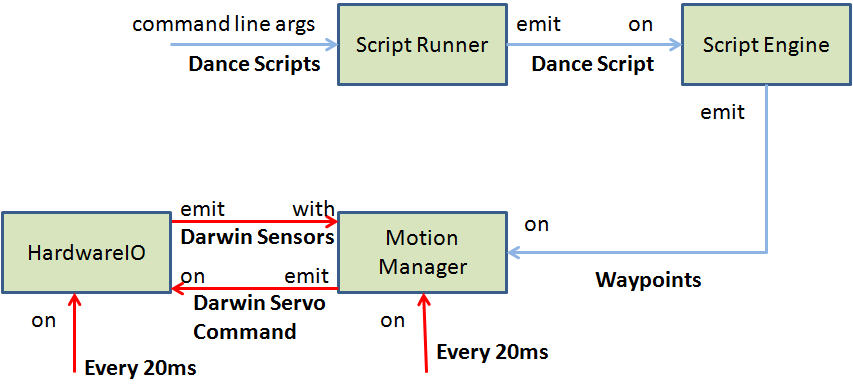
\includegraphics[scale=.5]{Presentation_Images/dance_script_new_arc.png}
			\caption{Components for Dancing to Script with Nuclear}
		\end{figure}
	\end{frame}	
	\begin{frame}
		\frametitle{Dancing and the New Architecture}
		\framesubtitle{Dancing to a Script}
		\begin{figure}
			\centering
			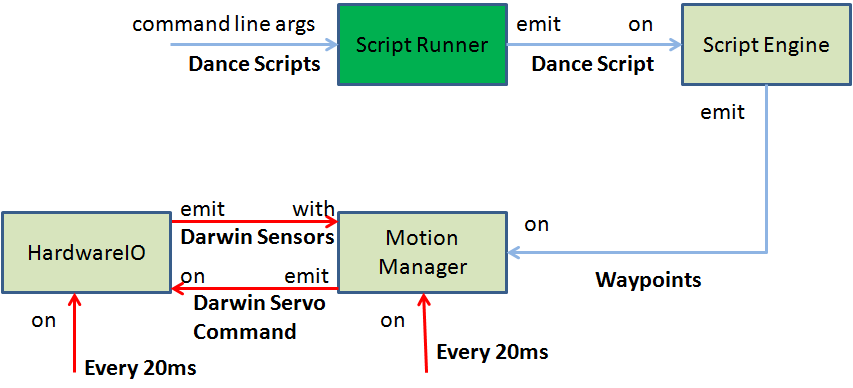
\includegraphics[scale=.5]{Presentation_Images/dance_script_new_arc_change.png}
			\caption{Components for Dancing to Script with Nuclear}
		\end{figure}
	\end{frame}
	\begin{frame}
		\frametitle{Dancing and the Old Architecture}
		\framesubtitle{Dancing to a Script}
		\begin{figure}
			\centering
			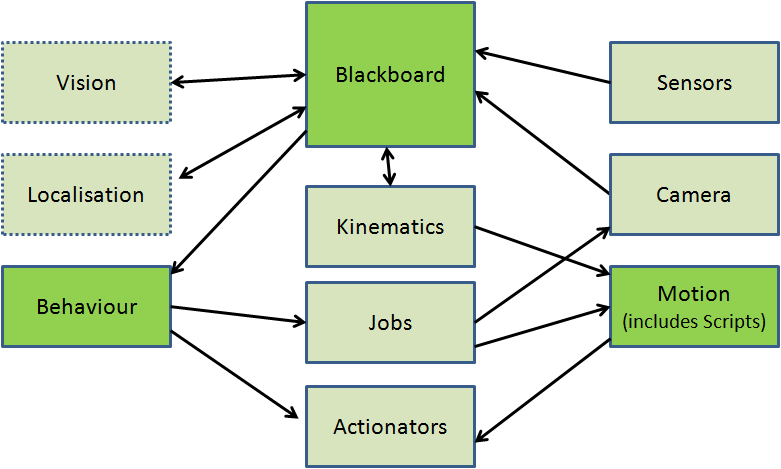
\includegraphics[scale=.45]{Presentation_Images/dance_script_old_arc.png}
			\caption{Components for Dancing to Script with the Old System}
		\end{figure}
	\end{frame}	
	\subsection{Dancing to Music} %-------------------
	\begin{frame}
		\frametitle{Dancing to Music}
		Things to consider:
		\begin{itemize}
			\item How to analyse music
			\begin{itemize}
				\item Holistic approach?
				\item Isolate musical characteristics?
			\end{itemize}
			\item Dance Moves
			\begin{itemize}
				\item Pre-Scripted or Dynamically Generated?
				\item Scope of movement. Involving legs or just upper body?
				\item How to relate dance moves to music
			\end{itemize}
		\end{itemize}
	\end{frame}	
	\begin{frame}
		\frametitle{Dancing to Music}
		\framesubtitle{Music Analysis}
		\begin{itemize}
			\item Beat is most important
			\item What is beat?
			\begin{itemize}
				\item Basic timing element of a song
				\item Tapping along to a song is finding the beat
			\end{itemize}
			\item Robot Dancing must be in time with beat
			\item Many other musical characteristics depend on beat
		\end{itemize}
	\end{frame}	
	\begin{frame}
		\frametitle{Dancing to Music}
		\framesubtitle{Finding the Beat}
		\begin{itemize}
			\item Finding the beat is known as Beat Tracking
			\item Beat Tracking must be:
			\begin{itemize}
				\item Real Time
				\item Predictive
				\item Quick
				\item Accurate
				\item Robust
			\end{itemize}
		\end{itemize}
	\end{frame}	
	\begin{frame}
		\frametitle{Dancing to Music}
		\framesubtitle{Beat and Dance}
		How we relate beat to dance:
		\begin{itemize}
			\item On Startup the dance Scripts are loaded
			\item When a beat is found, the Dance Engine is notified
			\item Each move in the dance script is reconfigured to be in time with the latest beat
			\item When no dance is currently being run, a new dance script is chosen to be run
		\end{itemize}
	\end{frame}	
	\begin{frame}
		\frametitle{Dancing and the New Architecture}
		\framesubtitle{Dancing to a Music}
		\begin{figure}
			\centering
			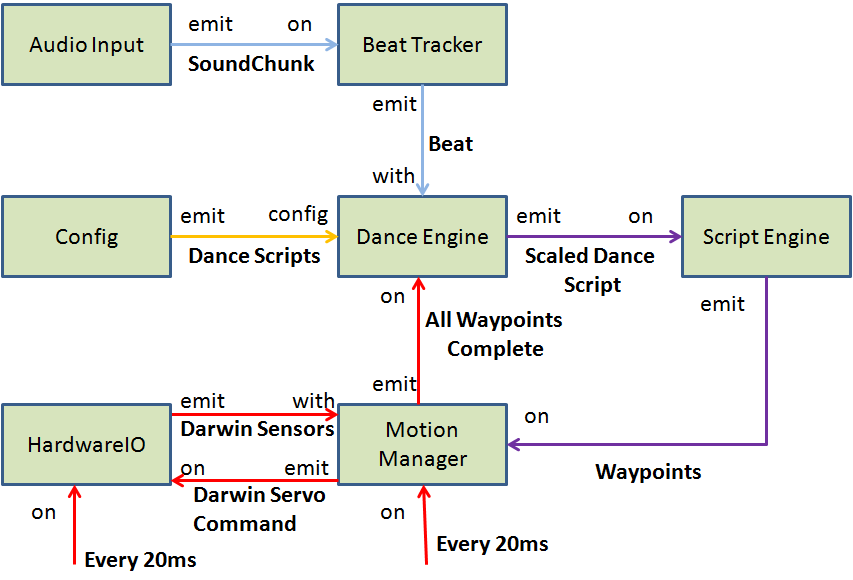
\includegraphics[scale=.45]{Presentation_Images/dance_audio_new_arc.png}
			\caption{Components for Dancing to Music with the NUClear}
		\end{figure}
	\end{frame}	
	\begin{frame}
		\frametitle{Dancing and the New Architecture}
		\framesubtitle{Dancing to a Music}
		\begin{figure}
			\centering
			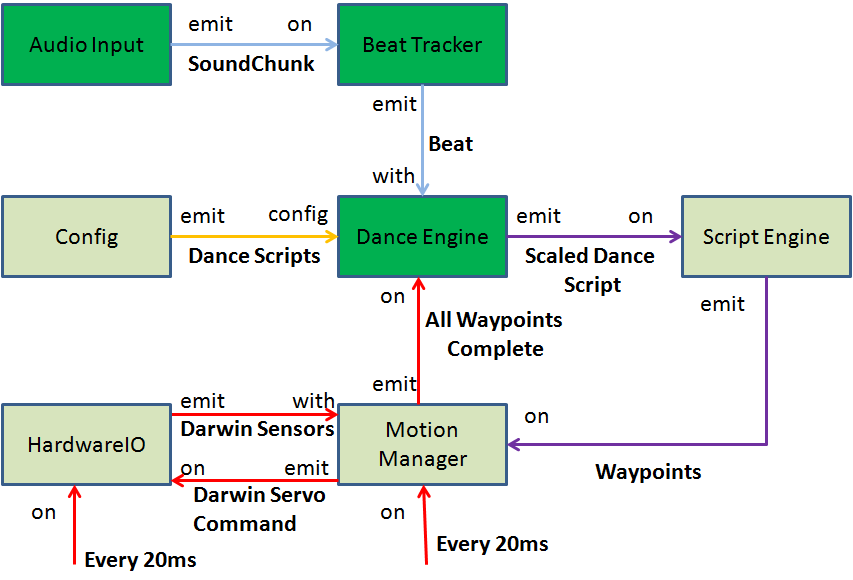
\includegraphics[scale=.45]{Presentation_Images/dance_audio_new_arc_change.png}
			\caption{Components for Dancing to Music with the NUClear}
		\end{figure}
	\end{frame}	
	\begin{frame}
		\frametitle{Dancing and the Old Architecture}
		\framesubtitle{Dancing to a Music}
		\begin{figure}
			\centering
			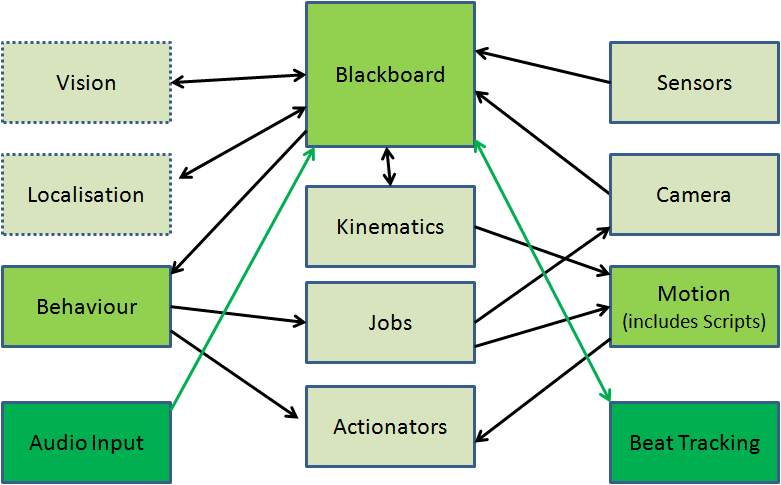
\includegraphics[scale=.45]{Presentation_Images/dance_audio_old_arc.png}
			\caption{Components for Dancing to Music with the Old System}
		\end{figure}
	\end{frame}	
	\subsection{Conclusions} %-------------------
	\begin{frame}
		\frametitle{Conclusions from Robot Dance}
			\begin{itemize}
				\item Robot Dance shows NUClear to be:
				\begin{itemize}
					\item Easy to learn
					\item Easy to use
					\item Modular
					\item Loosely Coupled
				\end{itemize}
			\end{itemize}
	\end{frame}	




%----------------------------------------------------------------------------------------
\section{Individual Research}
%----------------------------------------------------------------------------------------
\begin{frame}
	\sectionpage
\end{frame}

	%----------------------------------------------------------------------------------------
	\subsection{Overcoming Limits of Event Driven Systems}
	%----------------------------------------------------------------------------------------
	\begin{frame}
		\subsectionpage
	\end{frame}
	
	%----------------------------------------------------------------------------------------
	\subsection{Compile Time Message Routing}
	%----------------------------------------------------------------------------------------
	\begin{frame}
		\subsectionpage
	\end{frame}
	
	%----------------------------------------------------------------------------------------
	\subsection{Efficient Multithreading in Message Passing Systems}
	%----------------------------------------------------------------------------------------
	\begin{frame}
		\subsectionpage
	\end{frame}
	
	%----------------------------------------------------------------------------------------
	\subsection{Beat Detection}
	%----------------------------------------------------------------------------------------
	\begin{frame}
		\subsectionpage
	\end{frame}

\end{document} 
